\documentclass[svgnames]{beamer}
\mode<presentation>
\usefonttheme{serif}
\usecolortheme{dove}
\useinnertheme{rounded}
\setbeamercolor{item projected}{fg=black}
\setbeamertemplate{navigation symbols}{}

\usepackage[english]{babel}
\usepackage[latin1]{inputenc}
\usepackage{times}
\usepackage{amsmath}
\usepackage{amsfonts}
\usepackage{amssymb}
\usepackage{amsthm}
\usepackage{graphics}
\usepackage{multicol}
\usepackage{framed}
\usepackage{ulem}
\usepackage{ifthen}
\usepackage{tikz}
\usepackage{gastex}
\usepackage{ulem}
\usepackage{booktabs}

\newcommand{\buc}{\mathrm{B\ddot{u}chi}}
\newcommand{\bucf}{\buc(F)}
\newcommand{\bucfn}{\buc(F,N)}

\newcommand{\fin}{\mathrm{Fin}}
\newcommand{\bnd}{\mathrm{Bnd}}
\newcommand{\co}{\mathrm{Co}}

\newtheorem{conjecture}{Conjecture}

\newcommand{\set}[1]{\{ #1 \}}
\newcommand{\push}{\mathrm{push}}
\newcommand{\pop}{\mathrm{pop}}
\newcommand{\Skip}{\mathrm{skip}}

\newcommand{\parp}{\mathrm{Parity}}
\newcommand{\bound}{\mathrm{Bound}}

\newcommand{\W}{\mathcal{W}}
\newcommand{\WE}{\W_{E}}

\newtheorem{observation}{Observation}
\newtheorem{proposition}{Proposition}

\renewcommand{\ULthickness}{1.2pt}

%%%%%%%%%%%%%%%%%%%%%%%%%%%%%%%%%%%%%%%%%%%%%%%%%%%%%%%%%%%%%%%%%%%%%%%%%%%%%%%
%%%%%%%%%%%%%%%%%%%% A non-original creation by Nathana�l Fijalkow and myself %

\setbeamertemplate{frametitle}{%
  \vskip-2pt%
  \begin{beamercolorbox}[rightskip=2cm,leftskip=1em,dp=1ex,wd=12.8cm]{frametitle}%
    \vskip2pt%
    \usebeamercolor{frametitle}%
    \begin{tikzpicture}[scale=1]%
      \useasboundingbox (0,0) rectangle (0,0); %(-1,-1) rectangle (1,1);%
      \ifthenelse{\insertframenumber<\inserttotalframenumber}%
      { % uncomplete tart

        \pgfmathsetmacro{\aimangle}{90-(\insertframenumber*360/\inserttotalframenumber)}
        \fill [fill=frametitle.fg,thin, color=gray!50,draw=black] (11.8,.2) -- (11.8,.6) arc (90:\aimangle:0.4) -- cycle;%

      }{ % the full tart
        \fill[fill=frametitle.fg,thin, color=gray!50,draw=black] (11.8,0.2) circle (.4);%
      }%
      \fill[fill=frametitle.fg,thin, color=white,draw=black] (11.8,0.2) circle (.3);%
      \node at (11.8, .2) [black,circle]{\normalsize\insertframenumber};

    \end{tikzpicture}
    \insertframetitle%
    \vskip2pt%
  \end{beamercolorbox}%
}
%%%%%%%%%%%%%%%%%%%%%%%%%%%%%%%%%%%%%%%%%%%%%%%%%%%%%%%%%%%%%%%%%%%%%%%%%%%%%%%


\setbeamertemplate{blocks}[rounded]%
\setbeamercolor{block title}{bg=normal text.bg!90!black}
\setbeamercolor{block body}{bg=normal text.bg!95!black}

\AtBeginSection[]
{
\addtocounter{framenumber}{-1}
  \begin{frame}<beamer>{Outline}
    \tableofcontents[currentsection]
  \end{frame}
}

\AtBeginSubsection[]
{
\addtocounter{framenumber}{-1}
  \begin{frame}<beamer>{Outline}
    \tableofcontents[currentsection,currentsubsection]
  \end{frame}
}

\begin{document}

\addtocounter{framenumber}{-1}

\title{Boundedness games}
\author{Krishnendu Chatterjee \and Thomas Colcombet \and \underline{Nathana\"el Fijalkow} \and Florian Horn \and Denis Kuperberg \\
\and Micha{\l} Skrzypczak \and Martin Zimmermann}
\institute{Institute of Informatics, Warsaw University -- Poland 
\and LIAFA, Universit\'e Paris 7 Denis Diderot -- France}
\date{Highlights, September 19th, 2013}

\begin{frame}
\maketitle
\pause
This talk is about our \textit{joint} effort to understand  boundedness games.
\end{frame}

\begin{frame}{Motivation: expressing boundedness properties}
\begin{figure}[ht]
\begin{minipage}[b]{0.45\linewidth}
\centering
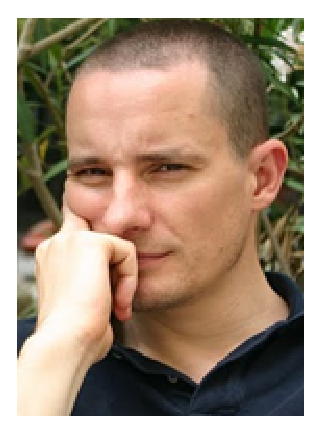
\includegraphics[width=19mm]{mikolaj}

$\mathrm{MSO} + \mathbb{U}$
\end{minipage}
\hspace{0.5cm}
\begin{minipage}[b]{0.45\linewidth}
\centering
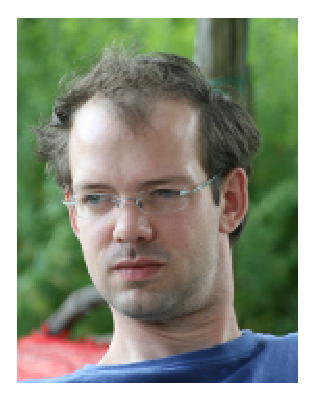
\includegraphics[width=20mm]{thomas}

$\mathrm{cost}\ \mathrm{MSO}$
\end{minipage}
\end{figure}
\begin{center}
A lot is known, and even more is not known about those two logics!
\end{center}
\end{frame}

\begin{frame}{Definition of boundedness games}
\begin{center}
\begin{multicols}{2}
\begin{picture}(40,60)(0,0)
	\gasset{Nw=8,Nh=8}
	
  	\rpnode[polyangle=45](1)(30,15)(4,5){}
  	\node(2)(20,30){}
  	\node(3)(40,30){}
  	\rpnode[Nmarks=i,iangle=180,polyangle=45](4)(0,30)(4,5){}
  	\rpnode[polyangle=45](5)(10,50)(4,5){}
  	\node(6)(10,10){}
  	\rpnode[polyangle=45](7)(30,50)(4,5){}

  	\drawedge(1,2){}
  	\drawedge[curvedepth=3](1,3){}
	\drawloop[loopangle=90](2){}
  	\drawedge(2,3){}
  	\drawedge(2,6){}
  	\drawedge[curvedepth=5](3,1){}
  	\drawedge(4,2){}
  	\drawedge[curvedepth=5](4,5){}
  	\drawedge[curvedepth=5](5,4){}
	\drawloop[loopangle=-90](6){}
  	\drawedge(7,5){}

\only<8,15>{
  	\rpnode[polyangle=45](1b)(30,15)(4,5){{\color{red}{$1$}}}
  	\node(2b)(20,30){{\color{blue}{$2$}}}
  	\node(3b)(40,30){{\color{red}{$3$}}}
  	\rpnode[Nmarks=i,iangle=180,polyangle=45](4b)(0,30)(4,5){{\color{red}{$3$}}}
  	\rpnode[polyangle=45](5b)(10,50)(4,5){{\color{blue}{$2$}}}
  	\node(6b)(10,10){{\color{blue}{$4$}}}
  	\rpnode[polyangle=45](7b)(30,50)(4,5){{\color{blue}{$0$}}}
}

\only<9,10,11,12,13,14,15>{
  	\drawedge(1,2){$i,\varepsilon$}
  	\drawedge[curvedepth=3](1,3){$\varepsilon,i$}
	\drawloop[loopangle=90](2){$i,i$}
  	\drawedge(2,3){$\varepsilon,\varepsilon$}
  	\drawedge[ELside=r](2,6){$i,r$}
  	\drawedge[curvedepth=5](3,1){$r,i$}
  	\drawedge(4,2){$\varepsilon,i$}
  	\drawedge[curvedepth=5](4,5){$\varepsilon,i$}
  	\drawedge[ELside=r,curvedepth=5](5,4){$i,i$}
	\drawloop[loopangle=-90](6){$\varepsilon,r$}
  	\drawedge[ELside=r](7,5){$i,\varepsilon$}
	}

\only<3,10>{\drawedge[AHLength=3,AHlength=4,linecolor=red,linewidth=0.7](4,2){}}
\only<5,12>{\drawedge[AHLength=3,AHlength=4,linecolor=red,linewidth=0.7](2,6){}}

\only<2,3,9,10>{\node[fillcolor=magenta,Nw=4,Nh=4](pebble)(0,30){}} 
\only<4,5,11,12>{\node[fillcolor=magenta,Nw=4,Nh=4](pebble)(20,30){}} 
\only<6,13>{\node[fillcolor=magenta,Nw=4,Nh=4](pebble)(10,10){}} 

\end{picture}
\begin{picture}(40,60)(0,0)
	\gasset{Nw=8,Nh=8}
	
\only<1,2,3,4,5,6>{
  	\node(Eve)(10,35){}
	\put(16,34){controlled by Eve}
  	\rpnode[polyangle=45](Adam)(10,25)(4,5){}
	\put(16,24){controlled by Adam}
	}

\only<8>{
	\begin{huge}
	\put(2,40){parity condition:}
	\put(-4,26){the minimal priority}
	\put(-4,18){seen infinitely often}
	\put(8,10){is even}
	\end{huge}
	}	

\only<9,10,11,12,13,14>{
	\begin{huge}
	\put(6,25){$\varepsilon: \textrm{nothing}$}
	\put(6,15){$i: \textrm{increment}$}
	\put(6,5){$r: \textrm{reset}$}
	\end{huge}
	}

\only<9,10>{
	\begin{huge}
	\put(10,50){$c_1 = 0$}
	\put(10,40){$c_2 = 0$}
	\end{huge}
}

\only<11,12>{
	\begin{huge}
	\put(10,50){$c_1 = 0$}
	\put(10,40){$c_2 = 1$}
	\end{huge}
}

\only<13,14>{
	\begin{huge}
	\put(10,50){$c_1 = 1$}
	\put(10,40){$c_2 = 0$}
	\end{huge}
}

\only<7,15>{
	\begin{huge}
	\put(-14,50){boundedness condition:}
	\put(12,36){parity}
	\put(15,28){and}
	\put(4,20){all counters}
	\put(3,12){are bounded}
	\end{huge}
}

\end{picture}
\end{multicols}
\end{center}
\end{frame}

\begin{frame}{Quantification}
Eve wins means:

\begin{figure}[ht]
\begin{minipage}[b]{0.45\linewidth}
\centering
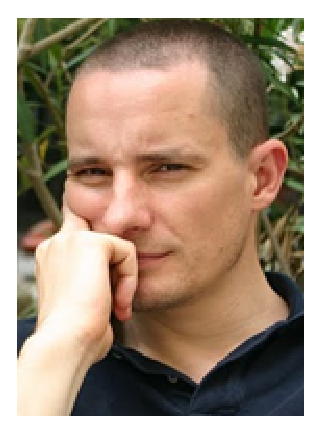
\includegraphics[width=19mm]{mikolaj}

$\exists \sigma$ (strategy for Eve),

$\forall \pi$ (paths), 

$\exists N \in \mathbb{N}$,

\end{minipage}
\hspace{0.5cm}
\begin{minipage}[b]{0.45\linewidth}
\centering
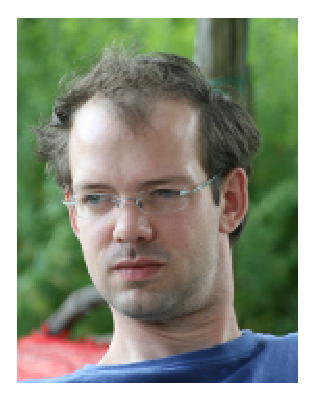
\includegraphics[width=20mm]{thomas}

$\exists \sigma$ (strategy for Eve),

$\exists N \in \mathbb{N}$,

$\forall \pi$ (paths),
\end{minipage}
\end{figure}
\begin{center}
$\pi$ satisfies parity
and each counter is bounded by $N$.
\end{center}

\pause
\begin{figure}[ht]
\begin{minipage}[b]{0.45\linewidth}
\centering

non-uniform

$(\mathrm{MSO} + \mathbb{U})$
\end{minipage}
\hspace{0.5cm}
\begin{minipage}[b]{0.45\linewidth}
\centering

uniform

$(\mathrm{cost}\ \mathrm{MSO})$
\end{minipage}
\end{figure}
\end{frame}


\begin{frame}{Research questions and some answers}
\begin{itemize}
	\item When are the two quantifications equivalent?
	\pause

	$\looparrowright$ Over pushdown arenas~[Chatterjee and F., 2013].
	\pause

\vskip1em	
	\item When is it decidable to determine the winner? efficient?
	\pause

	$\looparrowright$ Uniform quantifications, over finite arenas~[Colcombet and Loeding, 2009].

	$\looparrowright$ Non-uniform quantifications, parity games with cost~[F. and Zimmermann, 2012].
	\pause
	
\vskip1em	
	\item When does Eve has finite-memory winning strategies?
	\pause

	$\looparrowright$ Uniform quantifications, the B\"uchi case over infinite chronological arenas~[Vanden Boom, 2011].

	$\looparrowright$ Uniform quantifications, the parity case over thin tree arenas~[F., Horn, Kuperberg, Skrzypczak, unpublished].
\end{itemize}
\end{frame}

%\begin{frame}{Strategy (for Eve)}
%General form 
%$$\sigma : V^+ \rightarrow V$$
%\pause
%
%Positional or memoryless
%$$\sigma : V \rightarrow V$$
%\pause
%\begin{theorem}[M\"uller and Schupp]
%In parity games, both players have memoryless winning strategies.
%\end{theorem}
%\pause
%
%What about boundedness games?
%\pause
%
%\vskip1em
%Finite-memory 
%$$\left \{
%\begin{array}{c}
%\sigma : V \times M \rightarrow V \\
%\mu : M \times E \rightarrow M
%\end{array}
%\right.$$
%\end{frame}

\begin{frame}{Why finite-memory strategies?}
Thomas Colcombet's habilitation:
\vskip1em

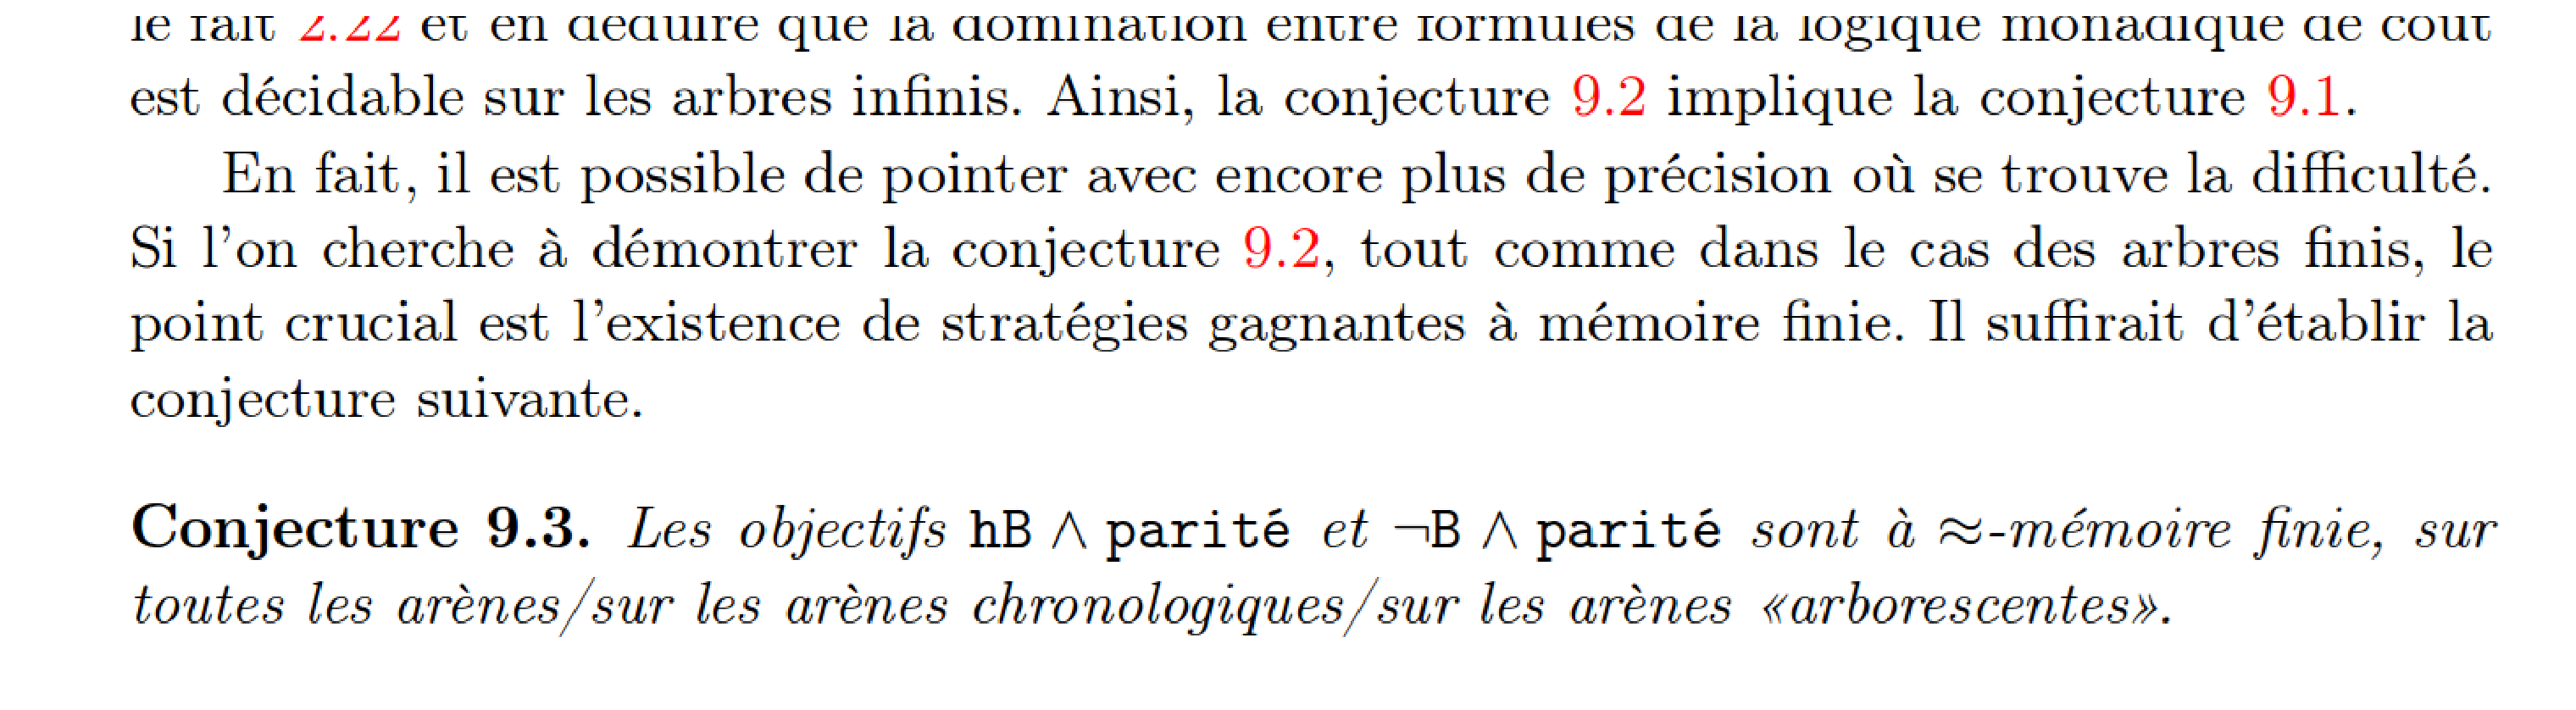
\includegraphics[width=100mm]{thomas_habilitation}

\vskip2em
Existence of finite-memory strategies in (some) boundedness games

$\Longrightarrow$ Decidability of cost MSO over infinite trees

$\Longrightarrow$ Decidability of the index of the non-deterministic Mostowski's hierarchy
(open for 40 years)!
\end{frame}

\begin{frame}{Working with potato trees}
\begin{figure}
	\begin{center}
	\begin{picture}(90,40)(0,-5)
	\gasset{Nw=7,Nh=7}

  	\node[linecolor=White](rootR)(47,38){}
  	\node[linecolor=White](0R)(17,18){}
  	\node[linecolor=White](1R)(77,18){}
  	\node[linecolor=White](00R)(2,-2){}
  	\node[linecolor=White](01R)(32,-2){}
  	\node[linecolor=White](10R)(62,-2){}
  	\node[linecolor=White](11R)(92,-2){}

  	\node[linecolor=White](rootL)(41,39){}
  	\node[linecolor=White](0L)(11,19){}
  	\node[linecolor=White](1L)(71,19){}
  	\node[linecolor=White](00L)(-4,-1){}
  	\node[linecolor=White](01L)(26,-1){}
  	\node[linecolor=White](10L)(56,-1){}
  	\node[linecolor=White](11L)(86,-1){}

  	\node[linecolor=White](root)(45,40){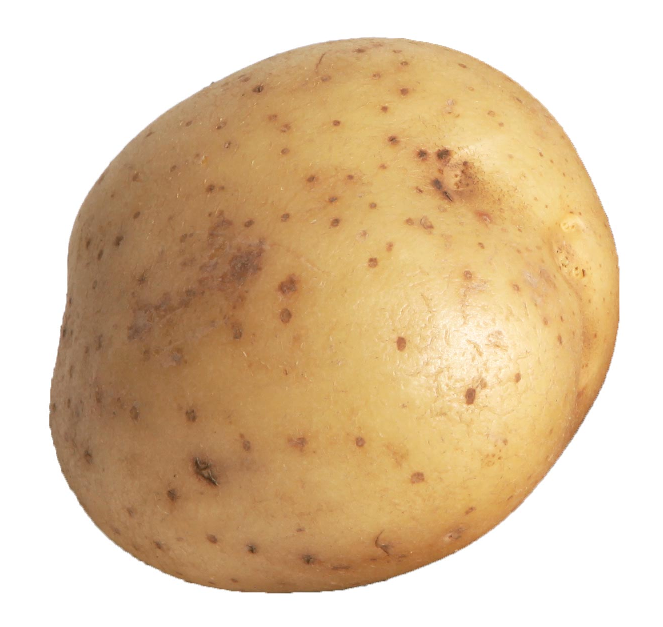
\includegraphics[width=12mm]{potato}}
  	\node[linecolor=White](0)(15,20){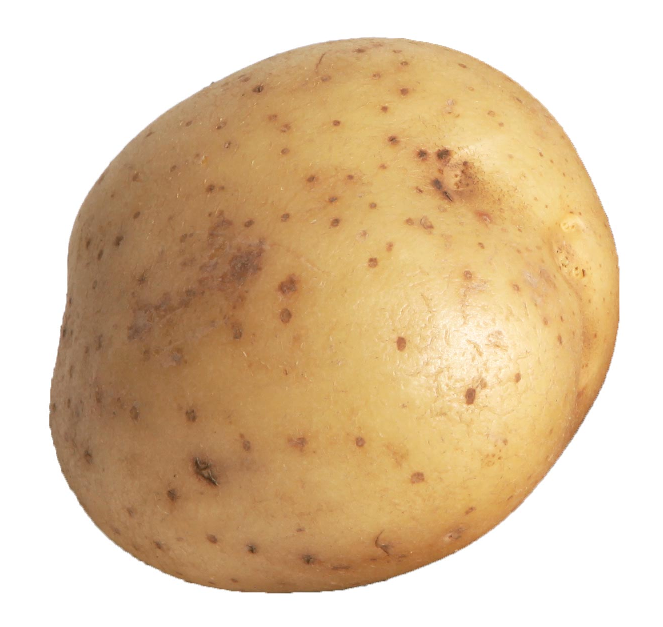
\includegraphics[width=12mm]{potato}}
  	\node[linecolor=White](1)(75,20){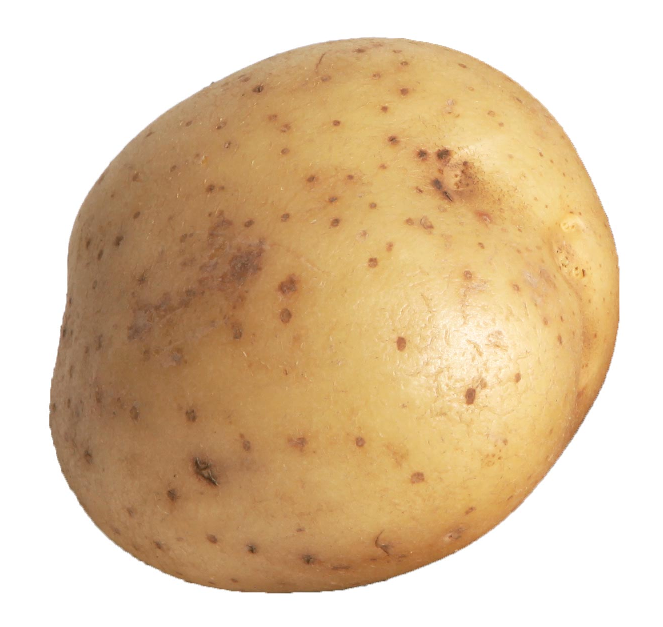
\includegraphics[width=12mm]{potato}}
  	\node[linecolor=White](00)(0,0){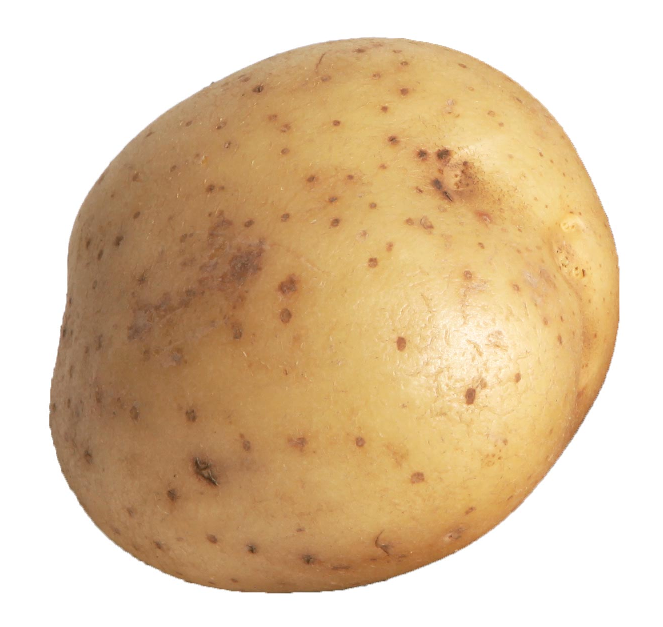
\includegraphics[width=12mm]{potato}}
  	\node[linecolor=White](01)(30,0){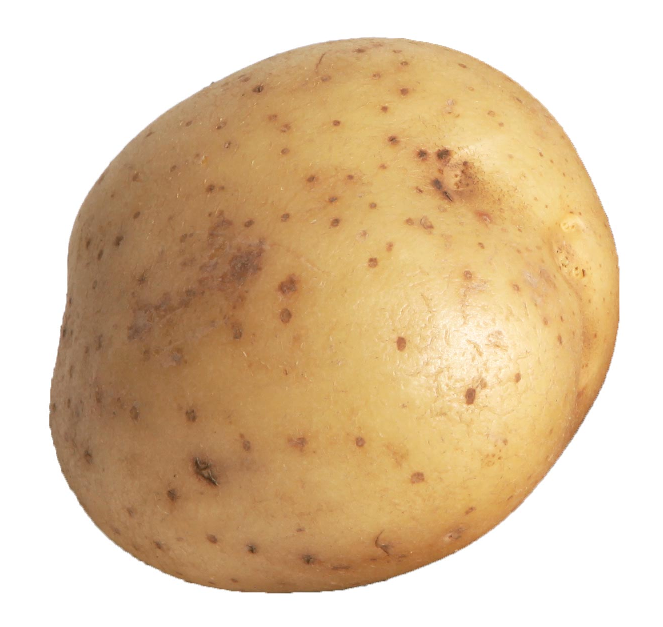
\includegraphics[width=12mm]{potato}}
  	\node[linecolor=White](10)(60,0){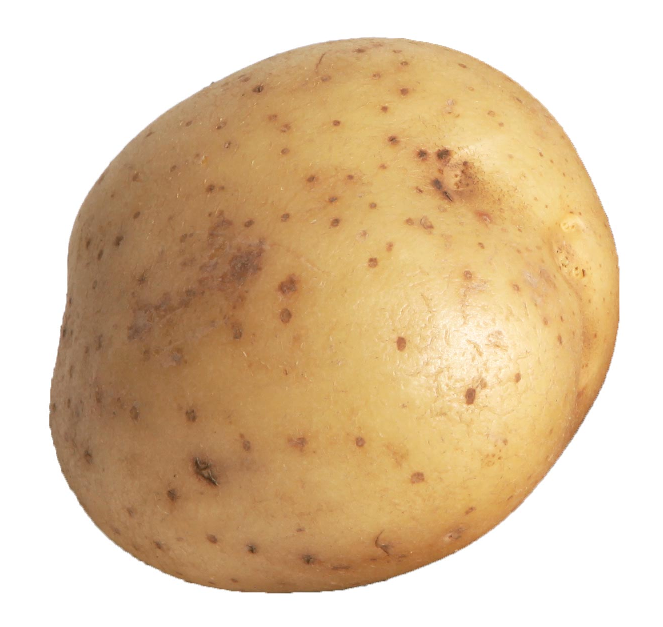
\includegraphics[width=12mm]{potato}}
  	\node[linecolor=White](11)(90,0){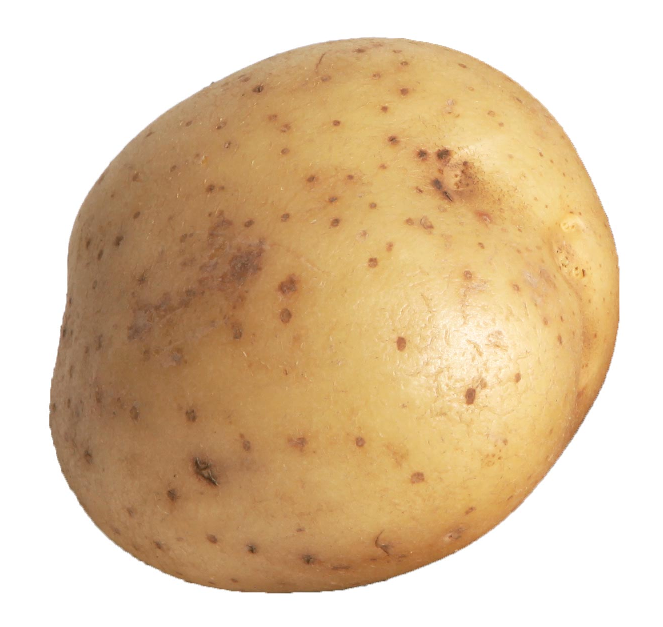
\includegraphics[width=12mm]{potato}}

  	\drawedge(root,0){}
  	\drawedge(root,1R){}
  	\drawedge(0,00L){}
  	\drawedge(0,01){}
  	\drawedge(1,10R){}
  	\drawedge(1,11L){}

  	\drawedge(rootR,0R){}
  	\drawedge(rootR,1L){}
  	\drawedge(0R,00){}
  	\drawedge(0R,01R){}
  	\drawedge(1R,10L){}
  	\drawedge(1R,11){}

  	\drawedge(rootL,0L){}
  	\drawedge(rootL,1){}
  	\drawedge(0L,00R){}
  	\drawedge(0L,01L){}
  	\drawedge(1L,10){}
  	\drawedge(1L,11R){}
	\end{picture}
	\end{center}
\end{figure}
\begin{theorem}[F., Horn, Kuperberg, Skrzypczak]
The $B$-part of Colcombet's conjecture holds for thin tree arenas!
\end{theorem}
\end{frame}



\end{document}

